\section{MIP model}\label{sec:malapertmipmodel}
As a baseline to compare other models' performance to, we first replicated
\section{Improved MIP model}\label{sec:improvedmipmodel}
Several improvements can be made to Malapert's MIP model in the form of
additional constraints shown in Model \ref{model:improvedmip}, as  
described in greater detail in the subsections below.

\begin{model}[h]
\begin{alignat}{2}
& \sum_{j \in J} x_{j,k-1} = 0 \rightarrow \sum_{j \in J} x_{jk} = 0 \quad &&
\forall k \in K \\
& e_k + \sum_{j \in J} x_{jk} \geq 1 \quad && \forall k \in K \\
& n_j (e_k-1) + \sum_{j \in J} x_{jk} \leq 0 \quad && \forall k \in K \\
& e_k - e_{k-1} \geq 0 \quad && \forall k \in K \\
& x_{jk} = 0 \quad && \forall \{j \in J, k \in K | j > k \} \\
& \Lmax \geq \big\lceil\frac{1}{b} \sum_{j} s_j
p_j\big\rceil - \delta_q \quad
&& \forall q, \forall \{ j \in J | d_j \leq \delta_q \}
\end{alignat}
\caption{Improvements to Malapert's original MIP model}
\label{model:improvedmip}
\end{model}

\subsection{Grouping empty batches} The given
formulation lacks a rule that ensures that no empty batch is followed by a
non-empty batch. Empty batches have no processing time and a due date only
bounded by $d_\text{max}$, so they can be sequenced between non-empty batches
without negatively affecting $\Lmax$. Since, however, desirable schedules have
no empty batches scattered throughout, we can easily reduce the search space by
disallowing such arrangements. The idea is illustrated in Figure
\ref{fig:dominancerule}.


\begin{figure}
  \centering
  \begin{subfigure}[b]{0.4\textwidth}
    \centering
    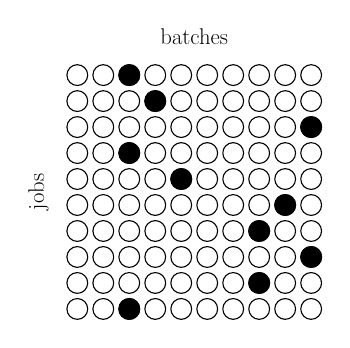
\begin{tikzpicture}[scale=0.33]
      \pgftext[x=-1.5cm, y=4.5cm, rotate=90]{\sansfont\Huge jobs}
      \pgftext[x=4.5cm, y=10.5cm]{\sansfont\Huge batches}

      \foreach \j in {0,...,9}
      {
        \foreach \k in {0,...,9}
        {
          \draw[] (\k, \j) circle [radius=0.4];
        }
      }
      \draw [fill] (2,0) circle [radius=0.4];
      \draw [fill] (2,6) circle [radius=0.4];
      \draw [fill] (2,9) circle [radius=0.4];
      \draw [fill] (3,8) circle [radius=0.4];
      \draw [fill] (4,5) circle [radius=0.4];
      \draw [fill] (7,1) circle [radius=0.4];
      \draw [fill] (7,3) circle [radius=0.4];
      \draw [fill] (8,4) circle [radius=0.4];
      \draw [fill] (9,2) circle [radius=0.4];
      \draw [fill] (9,7) circle [radius=0.4];
    \end{tikzpicture}
    \caption{Without dominance rule}
  \end{subfigure}
  \begin{subfigure}[b]{0.4\textwidth}
    \centering
    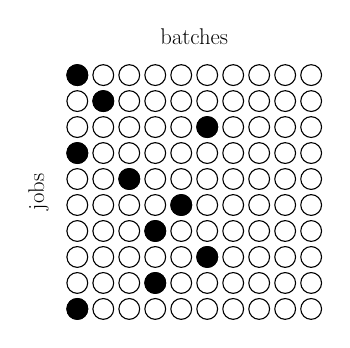
\begin{tikzpicture}[scale=0.33]
      \pgftext[x=-1.5cm, y=4.5cm, rotate=90]{\sansfont\Huge jobs}
      \pgftext[x=4.5cm, y=10.5cm]{\sansfont\Huge batches}

      \foreach \j in {0,...,9}
      {
        \foreach \k in {0,...,9}
        {
          \draw[] (\k, \j) circle [radius=0.4];
        }
      }
      \draw [fill] (0,0) circle [radius=0.4];
      \draw [fill] (0,6) circle [radius=0.4];
      \draw [fill] (0,9) circle [radius=0.4];
      \draw [fill] (1,8) circle [radius=0.4];
      \draw [fill] (2,5) circle [radius=0.4];
      \draw [fill] (3,1) circle [radius=0.4];
      \draw [fill] (3,3) circle [radius=0.4];
      \draw [fill] (4,4) circle [radius=0.4];
      \draw [fill] (5,2) circle [radius=0.4];
      \draw [fill] (5,7) circle [radius=0.4];
    \end{tikzpicture}
    \caption{With dominance rule}
  \end{subfigure}
\caption{Dominance rule to eliminate empty batches followed by non-empty batches
(circles represent the $x_{jk}$ variables; a filled circle stands for $x_{jk} =
1$)}\label{fig:dominancerule}
\end{figure}


A mathematical formulation is
\begin{alignat}{2}
& \sum_{j \in J} x_{j,k-1} = 0 \rightarrow \sum_{j \in J} x_{jk} = 0 \quad && \forall k \in K. \label{eq:emptybatch0}
\end{alignat}

To implement this, we can write constraints in terms of an additional  set of binary variables, $e_k$, indicating whether a batch $k$ is empty or not:

\begin{alignat}{2}
& e_k + \sum_{j \in J} x_{jk} \geq 1 \quad && \forall k \in K, \label{eq:emptybatch1} \\
& n_j (e_k-1) + \sum_{j \in J} x_{jk} \leq 0 \quad && \forall k \in K. \label{eq:emptybatch2}
\end{alignat}

Constraints \eqref{eq:emptybatch1} enforce $e_k = 1$ when the batch $k$ is
empty. Constraints \eqref{eq:emptybatch2} enforce $e_k = 0$ otherwise, since the
sum term will never exceed $n_j$. The rule \eqref{eq:emptybatch0} can now be
expressed as $e_{k-1} = 1 \rightarrow e_k = 1$, and implemented as follows:

\begin{alignat}{2}
& e_k - e_{k-1} \geq 0 \quad && \forall k \in K.
\end{alignat}

We can also prune any attempts to leave the first batch empty by adding a constraint $e_0 = 0$.


\subsection{No postponing of jobs to later batches}
Since the jobs are already sorted by non-decreasing due dates, it makes sense to explicitly instruct the solver never to attempt to push jobs into batches with a greater index than their own: even if every job had its own batch, it would be unreasonable to ever postpone a job to a later batch.
\begin{alignat}{2}
  & x_{jk} = 0 \quad && \forall \{j \in J, k \in K | j > k \} \label{eq:mipnopp}
\end{alignat}

\subsection[Lower bound on $\Lmax$]{Lower bound on {\sansitalicfont L}\textsubscript{max}}
Let a \textit{bucket} $q$ denote the set of all batches with due date $\delta_q$.
Then the completion date $C_q$ of this bucket is the completion date of the
last-scheduled batch with due date $\delta_q$, and the lateness of the bucket
$q$ is $L_q = C_q - \delta_q$. Since all batches up to and including those in
bucket $q$ are guaranteed to contain all jobs with due dates $d \leq \delta_q$
-- as ensured by the EDD ordering of batches -- the lower bound on every
bucket's lateness $LB(L_q)$ is a valid lower bound on $\Lmax$. In other words,
jobs with due date $d \leq \delta_q$ will be found only in batches up to and
including the last
batch of bucket $q$. This provides a lower bound on the lateness of bucket $q$:
\begin{alignat}{2}
& \Lmax \geq C_{\text{max},q} - \delta_q \quad && \forall q
\end{alignat}
The buckets up to bucket $q$ will likely also contain some later ($d >
\delta_q$) jobs in the optimal solution but this does not affect the validity of
the lower bound.

Now we need to find $C_{\text{max},q}$, or at least a lower bound on it, in
polynomial time. The simplest approach simply considers the jobs' total ``area''
(or ``energy''), i.e. the sum of all $s_j p_j$ products:
\begin{alignat}{2}
& C_{\text{max},q} \geq \big\lceil\frac{1}{b} \sum_{j} s_j
p_j\big\rceil \quad
&& \forall q, \forall \{ j \in J | d_j \leq \delta_q \}
\end{alignat}
A better lower bound on $C_{\text{max},q}$ would be given by a
preemptive-cumulative schedule. Unfortunately, minimizing $C_{\text{max}}$ for
such problems is equivalent to solving a standard bin-packing problem, which
requires exponential time.\footnote{In a preemptive-cumulative schedule, jobs
may be stopped and restarted mid-execution, but occupy a constant amount $s_j$
on the resource while executing. In such a schedule, minimizing the makespan is
as difficult as solving a bin-packing problem: we can break jobs into small
pieces (no longer than the smallest common divisor of the jobs' lengths $p$) and
then pack them together such as to minimize the number of small time slots
needed.}

